\documentclass[final,hyperref={pdfpagelabels=false}]{beamer}

\usetheme{rec}
\usepackage[orientation=portrait,size=a0,scale=1.7]{beamerposter} 
\usepackage[english]{babel} 
\usepackage{amsmath,amsthm,amssymb,latexsym}

\usefonttheme{professionalfonts}
\usefonttheme{serif}
\usepackage{fontspec}
\setmainfont{Ubuntu}

\usepackage{booktabs} 
\usepackage{xcolor}
\usepackage{fontawesome}
\usepackage{rotating}
\usepackage{graphicx}
\usepackage{multicol}



\newcommand*{\img}[1]{%
    \raisebox{-.1\baselineskip}{%
        \includegraphics[
        height=\baselineskip,
        keepaspectratio,
        ]{#1}%
    }%
}



\usecaptiontemplate{\small\structure{\insertcaptionname~\insertcaptionnumber: }\insertcaption} 
\boldmath 


%\title{\huge Age-structured contact networks, $R_0$ and COVID-19 } 
\title{\huge Temporal variability in population and community dynamics}
\author{Tad Dallas$^{1,2}$ \& Andrew Kramer$^{3}$}
\institute{$^{1}$ \ Department of Biological Sciences, Louisiana State University, USA \\ $^{2}$ \ Department of Biological Sciences, University of South Carolina, USA  \\ $^{3}$ \ Department of Integrative Biology, University of South Florida, USA} 



% footer text
\newcommand{\leftfoot}{} 
\newcommand{\rightfoot}{} 


\begin{document}

\begin{frame}[t] 

\begin{columns}[t] 

\begin{column}{0.02\textwidth}

\vspace{50cm}
\hspace{1.25cm}
\begin{rotate}{90}
    {\Large \faEnvelope} \ \ \  tad.a.dallas@gmail.com \ \ \ \textcolor{recRed}{$\vert$} \ \ \  
    {\Large \faDesktop}  \ \ \  taddallas.github.io \ \ \ \textcolor{recRed}{$\vert$} \ \ \
    {\LARGE \faGithubAlt}   \ \ \  taddallas 
\end{rotate}	

\end{column}





\begin{column}{0.02\textwidth}\end{column} % Empty spacer column


\begin{column}{0.46\textwidth} % The first column

	\begin{exampleblock}{main points}
    \vspace{0.5cm}
		\begin{itemize}
			\item Community variability is less than mean population variability in simulated data, but not in empirical data. 
			\item There is a latitudinal signal in population and community temporal variability, and differences as a function of habitat type.
		\end{itemize} 
	\end{exampleblock}


  \vspace{1cm}

	\begin{alertblock}{Setup and question}
  \bigskip
  Populations and communities fluctuate in their overall numbers through time, and the magnitude of fluctuations in individual species may scale to communities. However, the composite variability at the community scale is expected to be tempered by opposing fluctuations in individual populations, a phenomenon often called the \textit{portfolio effect}. 

	\end{alertblock}




		\begin{figure}
			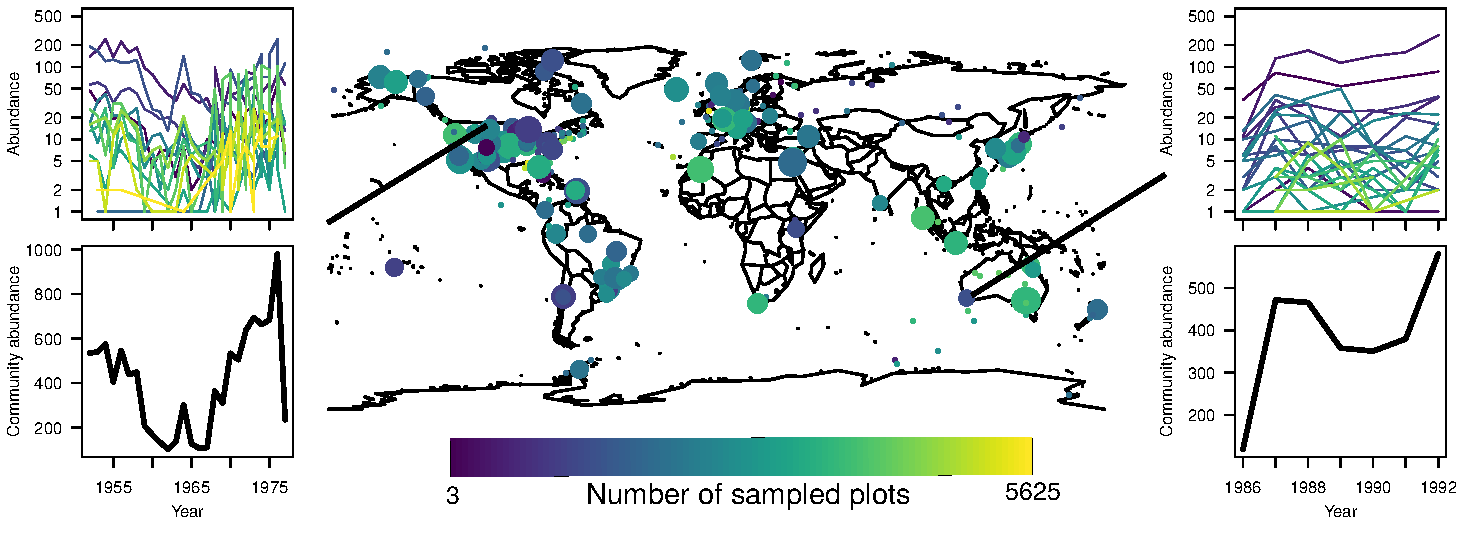
\includegraphics[width=\linewidth]{figures/conceptFigure.pdf}
			\caption{ \ Plotted points are mean latitude and longitude values for given sampled locations, where point size is proportional to species richness and point color corresponds to the number of sampled plots per site. }
		\end{figure}



	\begin{block}{Big questions}

		\begin{itemize}
			\item Do we see evidence for portfolio effects in empirical community time series data?
			\item Are there differences among habitat types or across space in population and community temporal variability?
		\end{itemize}
	\end{block}



\begin{alertblock}{Methods}
	\begin{itemize}
		\item BioTime database (n=361 communities at \textit{study} level)
		\item Simulated data (Ricker model with random growth rates $R$ and intraspecific competition coefficients $\alpha_i$)
	\end{itemize}

  \begin{equation}
  \label{eq:ricker}
  N_{t+1} = N_{t} \ R \ e^{- \alpha N_{t}}
  \end{equation}

 Sampled the potential space of non-interacting species in terms of: 
 \begin{itemize}
   \item population growth rate $R$ [0.9 - 2.5] 
   \item intraspecific competition $\alpha$ [0.0001 - 0.1] 
 \end{itemize}
 to build communities of between 2 and 40 species
\end{alertblock}








\end{column} 







\begin{column}{0.02\textwidth}\end{column} % Empty spacer column






\begin{column}{0.46\textwidth} 



\begin{exampleblock}{Measuring temporal variability}
\begin{equation}
  D = \frac{1}{n-1} \sum_{t=1}^{n-1} \left\lvert ln\left( \frac{p_{t+1}+k}{p_{t}+k}\right)\right\rvert
\end{equation}

\vspace{0.5cm}
where $p_{t}$ corresponds to abundance at time $t$, where the entire length of the time series is $n$, and $k$ is a constant.

\end{exampleblock}




\begin{alertblock}{Temporal variability across space and habitat type}

		\begin{figure}
			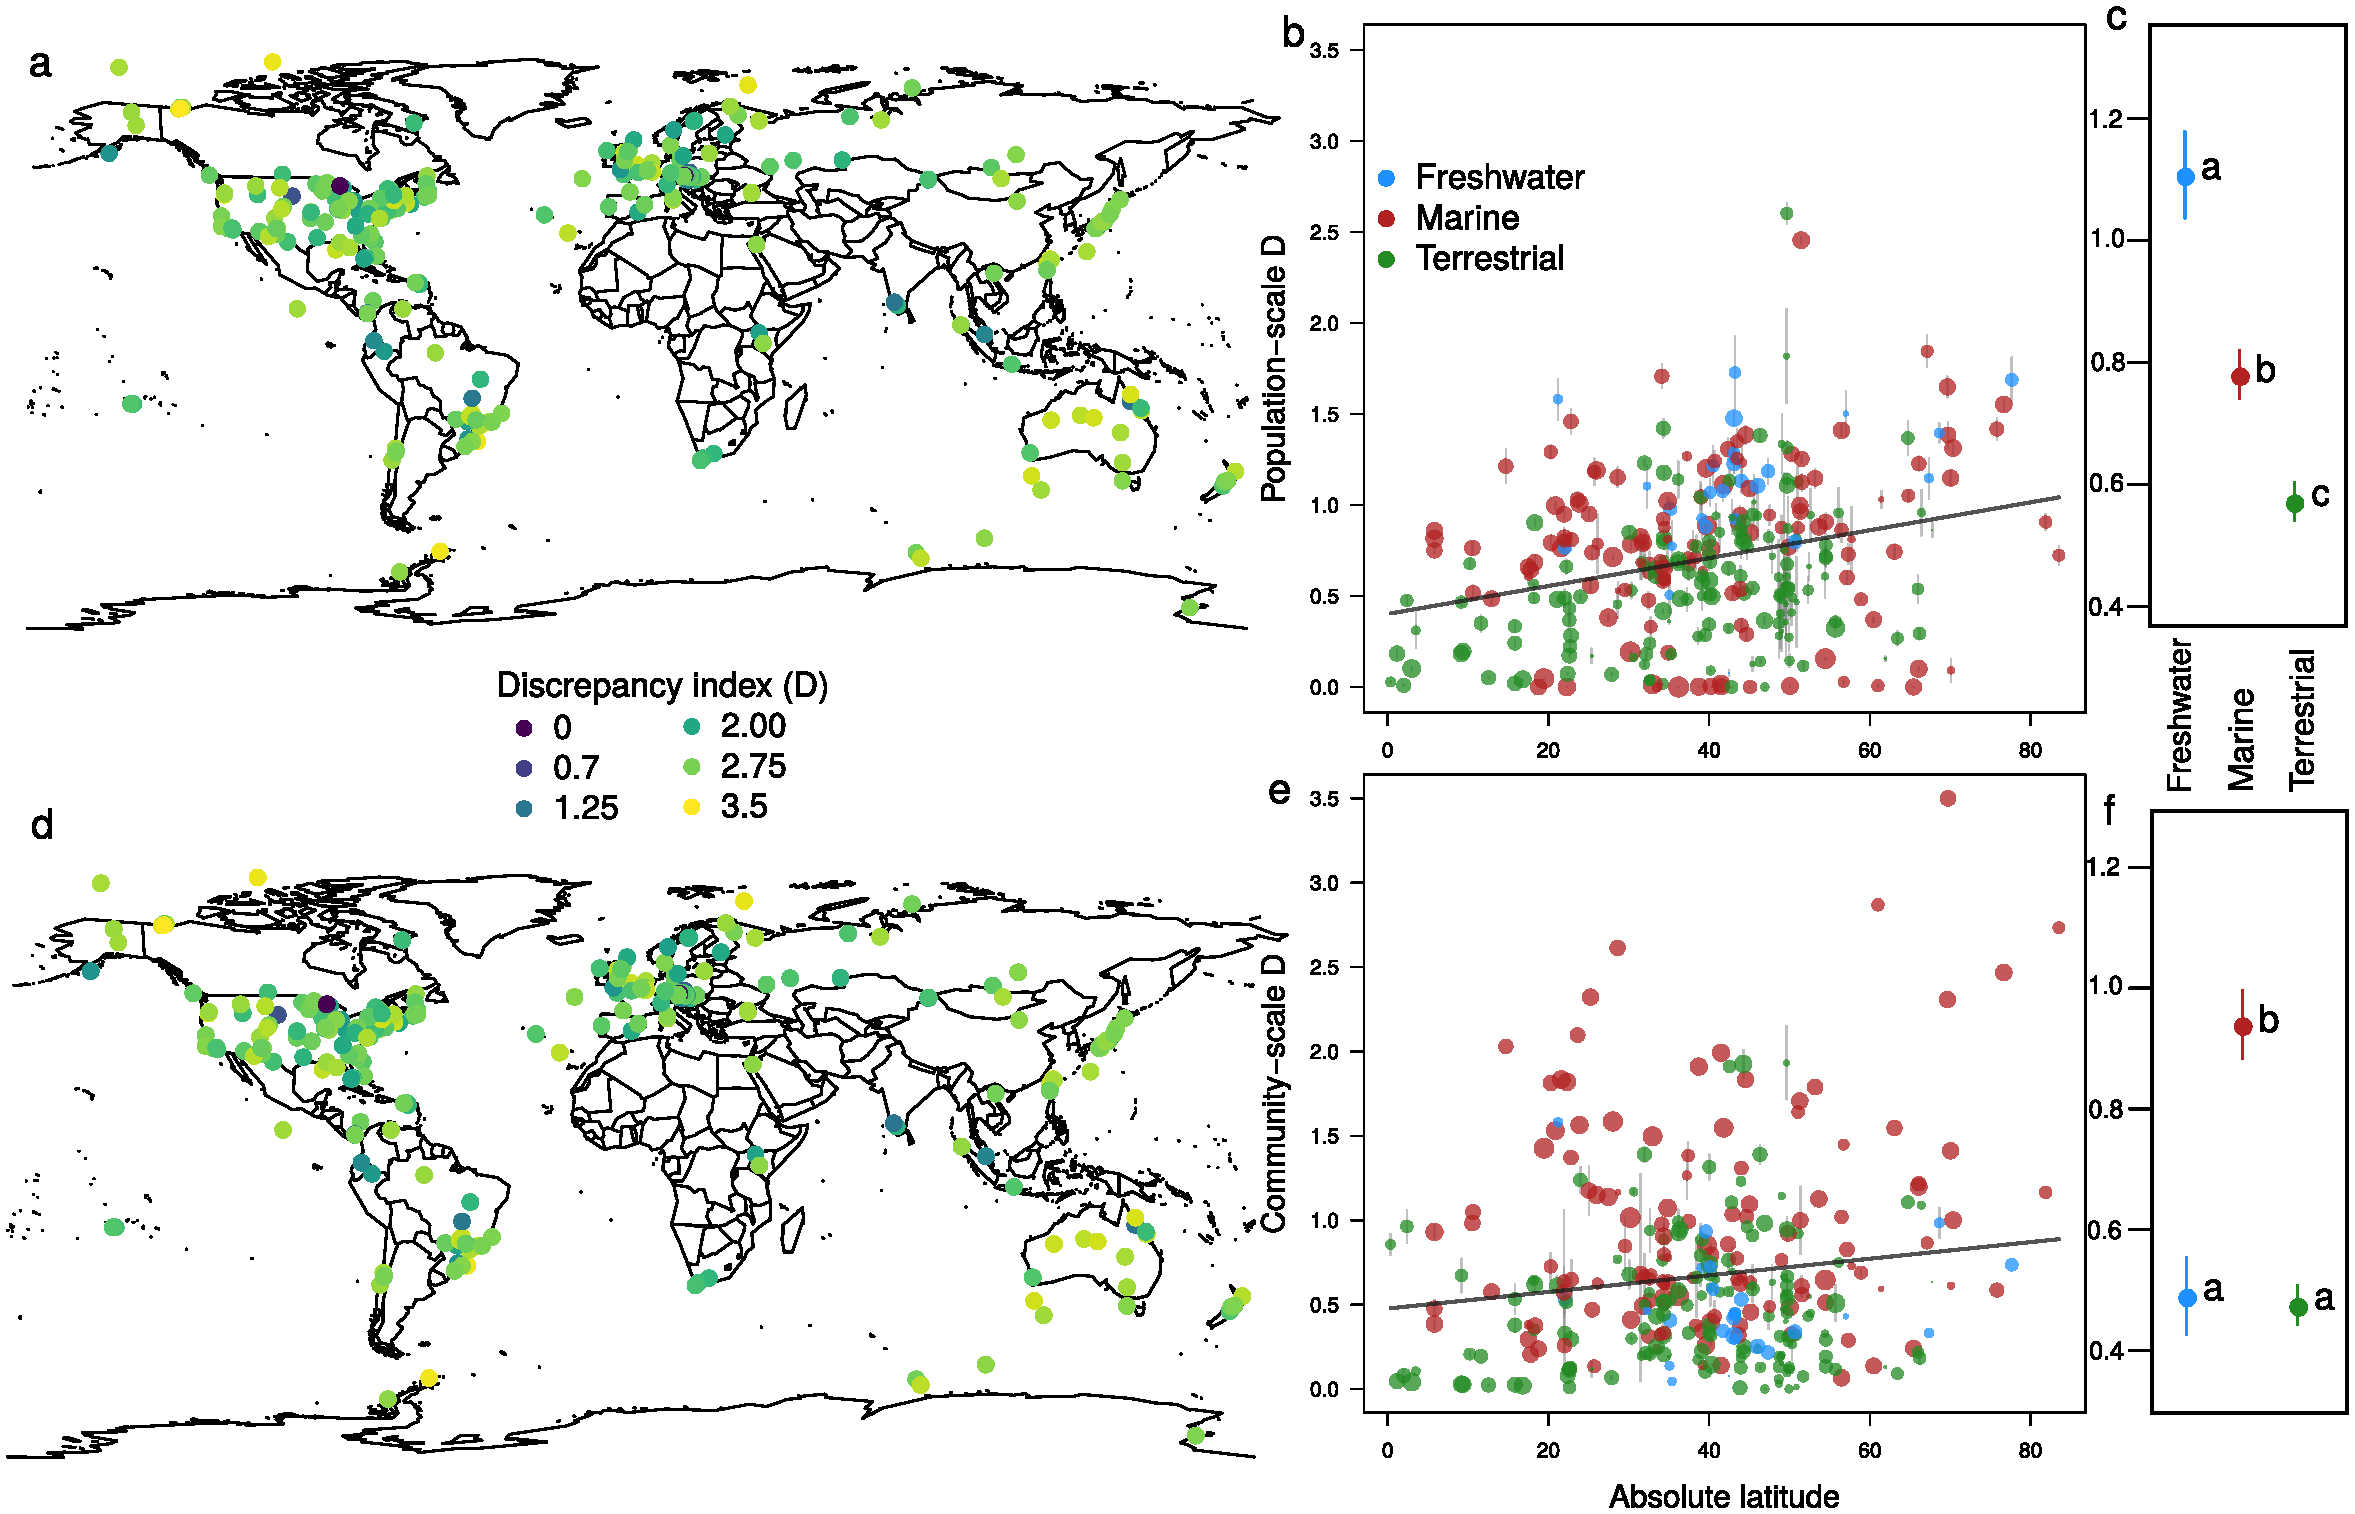
\includegraphics[width=\linewidth]{figures/stabilityMapD.pdf}
			\caption{ \ The spatial distribution of population (panel \texttt{a}) and community (panel \texttt{d}) temporal variability. Point size in panels \texttt{b} and \texttt{e} are proportional to the number of species present.}
		\end{figure}
\end{alertblock}


	\begin{block}{Portfolio effects in simulated and empirical data}

		\begin{figure}
			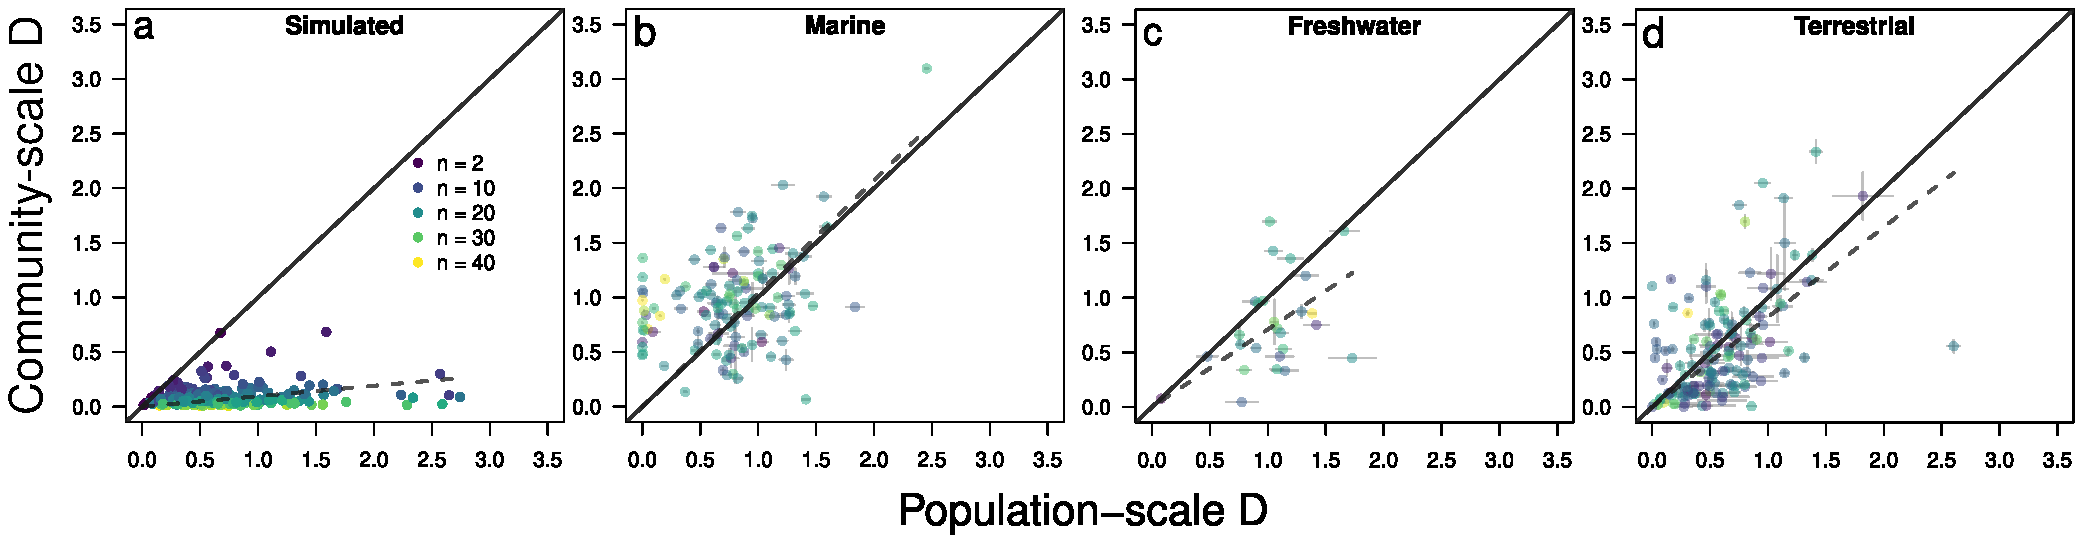
\includegraphics[width=\linewidth]{figures/dSpStudy.pdf}
			\caption{The relationship between temporal variability ($D$) at population (x-axis) and community (y-axis) scales, using a theoretical model assuming no species interactions (\texttt{a}) and in empirical communities across aquatic (\texttt{b}), marine (\texttt{c}), and terrestrial (\texttt{d}) environments. While generally positive, suggesting that temporal variability in populations scales to communities, the relationship is quite variable.}
		\end{figure}

	\end{block}



\begin{exampleblock}{What does this mean?}

\begin{itemize}
  \item Portfolio effects may vary in their strength across communities in different environments, different latitudes, and with different numbers of species. 
  \item Simulated communities aren't real communities. Nature != relatively neutral? 
  \item The results are the same if we use a measure of stability that doesn't consider temporal order.
\end{itemize}
\end{exampleblock}


\end{column} 


\begin{column}{0.02\textwidth}\end{column} % Empty spacer column
\end{columns} 


{\Huge \faThumbsOUp} This work has been supported by the U.S. National Science Foundation grant (NSF-DEB-2017826). \textcolor{recRed}{Thank you!}  

\end{frame} 


\end{document}
